\documentclass{beamer}

\usetheme{Warsaw}
%\usetheme{CambridgeUS}

% modification history
% created on 18 sep 2011
% modified on 25 mar

%\usepackage{amsfonts, amsmath, amssymb}

%\setbeamertemplate{theorems}[numbered]
%\setbeamertemplate{theorems}[ams style] 
\usepackage[skins,breakable]{tcolorbox}
%\usepackage[normalem]{ulem}

%\usefonttheme[onlymath]{serif}                     // change the style of math font 

%=============set slide number=================
\addtobeamertemplate{navigation symbols}{}{
    \usebeamerfont{footline}
    \usebeamercolor[fg]{footline}
    \hspace{1em}
    \insertframenumber/\inserttotalframenumber
}
\setbeamercolor{footline}{fg=black}
\setbeamerfont{footline}{series=\bfseries}


%=============set footline=====================
\setbeamertemplate{footline}
{
  \leavevmode%
  \hbox{%
  \begin{beamercolorbox}[wd=.55\paperwidth,ht=2.25ex,dp=1ex,center]{author in head/foot}%
    \usebeamerfont{author in head/foot}\insertshortauthor
  \end{beamercolorbox}%
  \begin{beamercolorbox}[wd=.45\paperwidth,ht=2.25ex,dp=1ex,center]{title in head/foot}%
    \usebeamerfont{title in head/foot}\insertshorttitle
  \end{beamercolorbox}}%
  \vskip0pt%
}

%creating a rectangle box def
\newtcbox{\mybox}[1][red]{arc=0pt,outer arc=0pt,colback=#1!10!white,colframe=#1!50!black, boxsep=0pt,left=1pt,right=1pt,top=2pt,bottom=2pt,boxrule=0pt,bottomrule=1pt,toprule=1pt}

\newtcbox{\xmybox}[1][red]{arc=7pt,colback=#1!10!white,colframe=#1!50!black,before upper={\rule[-3pt]{0pt}{10pt}},boxrule=1pt,boxsep=0pt,left=6pt,right=6pt,top=2pt,bottom=2pt}
%the ``on line'' option doesn't work. so omitting it

%===== spacing =====

\def\extraspacing{\vspace{2mm} \noindent}
\def\vgap{\vspace{2mm}}
\def\hgap{\textrm{\hspace{1mm}}}

%===== tabbing =====

\def\tab{\hspace{2mm}}
\def\tabpos{\hspace{4mm} \= \hspace{4mm} \= \hspace{4mm} \= \hspace{4mm} \=
\hspace{4mm} \= \hspace{4mm} \= \hspace{4mm} \= \hspace{4mm} \= \hspace{4mm}
\kill}
\newcommand{\mytab}[1]{\begin{tabbing}\tabpos #1\end{tabbing}}

%===== blocks =====

% \newtheorem{theorem}{Theorem}
% \newtheorem{lemma}{Lemma}
% \newtheorem{corollary}{Corollary}
% \newtheorem{proposition}{Proposition}
% \newtheorem{definition}{Definition}
% \newtheorem{problem}{Problem}

\newcommand{\cbox}[2]{\begin{tcolorbox}[arc=0mm, colframe=#1!50!black, colback=#1!10!white]#2\end{tcolorbox}}
\newcommand{\minipg}[2]{\begin{center}\begin{minipage}{#1}#2\end{minipage}\end{center}}
\newcommand{\myfrm}[1]{\begin{frame}\begin{small}#1\end{small}\end{frame}} 
\newcommand{\myitems}[1]{\begin{itemize}#1\end{itemize}}
\newcommand{\myenums}[1]{\begin{enumerate}#1\end{enumerate}}
\newcommand{\myfig}[1]{\begin{figure}\centering #1\end{figure}}
    
%===== math macros =====
\newcommand{\bm}[1]{\textrm{\boldmath${#1}$}}
%\newcommand{\smat}[2]{\left[\begin{tabular}{#1}#2\end{tabular}\right]}
%\newcommand{\bmat}[2]{\left|\begin{tabular}{#1}#2\end{tabular}\right|}
\newcommand{\bmat}[1]{\begin{bmatrix}#1\end{bmatrix}}
\newcommand{\vmat}[1]{\begin{vmatrix}#1\end{vmatrix}}
\newcommand{\myeqn}[1]{\begin{eqnarray}#1\end{eqnarray}}
\newcommand{\set}[1]{\{#1\}}

\def\eps{\epsilon}
\def\fr{\frac}
\def\lc{\lceil}
\def\lf{\lfloor}
\def\rc{\rceil}
\def\rf{\rfloor}
\def\Pr{\textrm{\boldmath$Pr$}}
\def\expt{\textrm{\boldmath$E$}}
\def\real{\mathbb{R}}
\def\int{\mathbb{Z}}
\def\*{\star}
\def\tO{\tilde{O}}

\DeclareMathOperator*{\argmin}{arg\,min}
\DeclareMathOperator*{\polylg}{polylg}
\DeclareMathOperator*{\polylog}{polylog}
\DeclareMathOperator*{\intr}{\cap}

\def\nn{\nonumber}
\def\mit{\mathit}


%===== misc =====

\def\done{\hspace*{\fill} $\framebox[2mm]{}$}	% end of proof
\def\ttt{\texttt}

%===== coloring =====
\newcommand{\red}[1]{\textcolor{red}{#1}}
\newcommand{\bred}[1]{\textcolor{red}{\bf #1}}
\newcommand{\blue}[1]{\textcolor{blue}{\bf #1}}

\usepackage{color}
\usepackage{graphicx}
\usepackage{multirow}
\usepackage{wrapfig}
\usepackage[skins,breakable]{tcolorbox}

\def\done{\hfill$\square$}
\def\ttt{\texttt}
\def\vgap{\vspace{5mm}}

\def\abt{\ttt{ABORT}}
\def\best{\mit{best}}
\def\cmt{\ttt{COMMIT}}
\def\ins{\ttt{INSERT}}
\def\rd{\ttt{READ}}
\def\size{\mit{size}}
\def\sort{\mit{sort}}
\def\wt{\ttt{WRITE}}

\title[DATABASE SYSTEM PRINCIPLES]{Transactions 3:\\ Serializability}

\author[Yufei Tao @ NTU]{Yufei Tao}
\institute[]{\url{https://www.cse.cuhk.edu.hk/~taoyf}}
\date{}

% \def\dtm{\mathit{d\mbox{-}tm}}
% \def\ftm{\mathit{f\mbox{-}tm}}
\def\bestext{\mathit{best\mbox{-}ext}}

\begin{document}
%-------------------------------------------------------------
\begin{frame}
    \titlepage
%     \begin{tcolorbox}[arc=0mm, colframe=green!50!black, colback=green!10!white] 
%     \end{tcolorbox}
\end{frame}
%-------------------------------------------------------------
\begin{frame}
\begin{small}
    This lecture focuses on \bred{serializable schedules}. We will learn a conservative method to check whether a schedule is serializable.

    \vgap

    Recall:
    \cbox{blue}{
        A schedule is \blue{serializable} if it is equivalent to \bred{some} serial schedule. Otherwise, it is \blue{non-serializable}.
    }
\end{small}    
\end{frame}
%-------------------------------------------------------------
\myfrm{
    \cbox{green}{
        \blue{Example:} The following schedule is serializable.
        \begin{center}
        \begin{tabular}{c|c|c}
            & $\red{T_1}$ & $\red{T_2}$\\
            \hline
            1&& \rd($A$) \\
            2&& $A = A + 1$ \\
            3&& \wt($A$) \\
            4&\rd($A$) & \\
            5&$B = A$ & \\
            6&\wt($B$) &\\
            7&& \cmt \\
            8&\cmt &
        \end{tabular}
        \end{center}

        It is equivalent to the serial schedule $(T_2, T_1)$, but \bred{not} equivalent to the serial schedule $(T_1, T_2)$.
    }
}
%-------------------------------------------------------------
\myfrm{
    \cbox{green}{
        \blue{Example:} The following schedule is non-serializable.

        \begin{center}
        \begin{tabular}{c|c|c}
            &$\red{T_1}$ & $\red{T_2}$\\
            \hline
            1&\rd($A$) & \\
            2&$A = A + 1$ &\\
            3&& \rd($A$) \\
            4&& $A = A + 1$ \\
            5&\wt($A$) & \\
            6&& \wt($A$) \\
            7&& \cmt \\
            8&\cmt &
        \end{tabular}
        \end{center}

        \vgap

        If $A$ was 0 before running the schedule, what is its value afterwards?
    }
}
%-------------------------------------------------------------
\myfrm{
    \cbox{blue}{
        Let $\red{I_1}$ and $\red{I_2}$ be instructions in a schedule that belong to different transactions. They are in \blue{conflict} if \bred{one} of the following is true:
        \myitems{
            \item $I_1 = \red{\rd(X)}$ and $I_2 = \red{\wt(X)}$ for some value $X$;
            \item $I_1 = \red{\wt(X)}$ and $I_2 = \red{\rd(X)}$ for some value $X$;
            \item $I_1 = \red{\wt(X)}$ and $I_2 = \red{\wt(X)}$ for some value $X$.
        }
    }

}
%-------------------------------------------------------------
\myfrm{
    \cbox{green}{
        \blue{Example:}
        \begin{center}
        \begin{tabular}{c|c|c}
            &$\red{T_1}$ & $\red{T_2}$\\
            \hline
            1&\rd($A$) & \\
            2&$A = A + 1$ &\\
            3&& \rd($A$) \\
            4&& $A = A + 1$ \\
            5&\wt($A$) & \\
            6&& \wt($A$) \\
            7&& \cmt \\
            8&\cmt &
        \end{tabular}
        \end{center}

        Instructions 1 and 6 are in conflict. \\
        Instructions 3 and 5 are in conflict. \\
        Instructions 5 and 6 are in conflict.
    }
}
%-------------------------------------------------------------
\myfrm{
    \xmybox{Precedence Graph}

    \vgap

    $\red{\Sigma:}$ a schedule involving $k \ge 2$ transactions $\red{T_1}, ..., \red{T_k}$.

    \vgap

    \cbox{blue}{
        The \blue{precedence graph} of $\Sigma$ is a directed graph $\red{G = (V, E)}$ where
        \myitems{
            \item $V = \set{T_1, T_2, ..., T_k}$ (i.e., one vertex per transaction);
            \item $E$ contains an edge from $\red{T_i}$ to $\red{T_j}$ if and only if $\Sigma$ has two \bred{conflicting} instructions $\red{I_1}$ and $\red{I_2}$ such that
            \myitems{
                \item $I_1$ precedes $I_2$ in $\Sigma$, and
                \item $I_1$ belongs to $T_i$ and $I_2$ belongs to $T_j$.
            }
        }
    }
}
%-------------------------------------------------------------
\myfrm{
    \cbox{green}{
        \blue{Example:}

        \vgap

        \begin{tabular}{cc}
            \begin{minipage}{0.47\linewidth}
                \begin{tabular}{c|c|c}
                    &$\red{T_1}$ & $\red{T_2}$\\
                    \hline
                    1&\rd($A$) & \\
                    2&$A = A + 1$ &\\
                    3&& \rd($A$) \\
                    4&& $A = A + 1$ \\
                    5&\wt($A$) & \\
                    6&& \wt($A$) \\
                    7&& \cmt \\
                    8&\cmt &
                \end{tabular}
            \end{minipage}
            &
            \begin{minipage}{0.47\linewidth}
                \begin{center}
                    Precedence graph: \\[1mm]
                    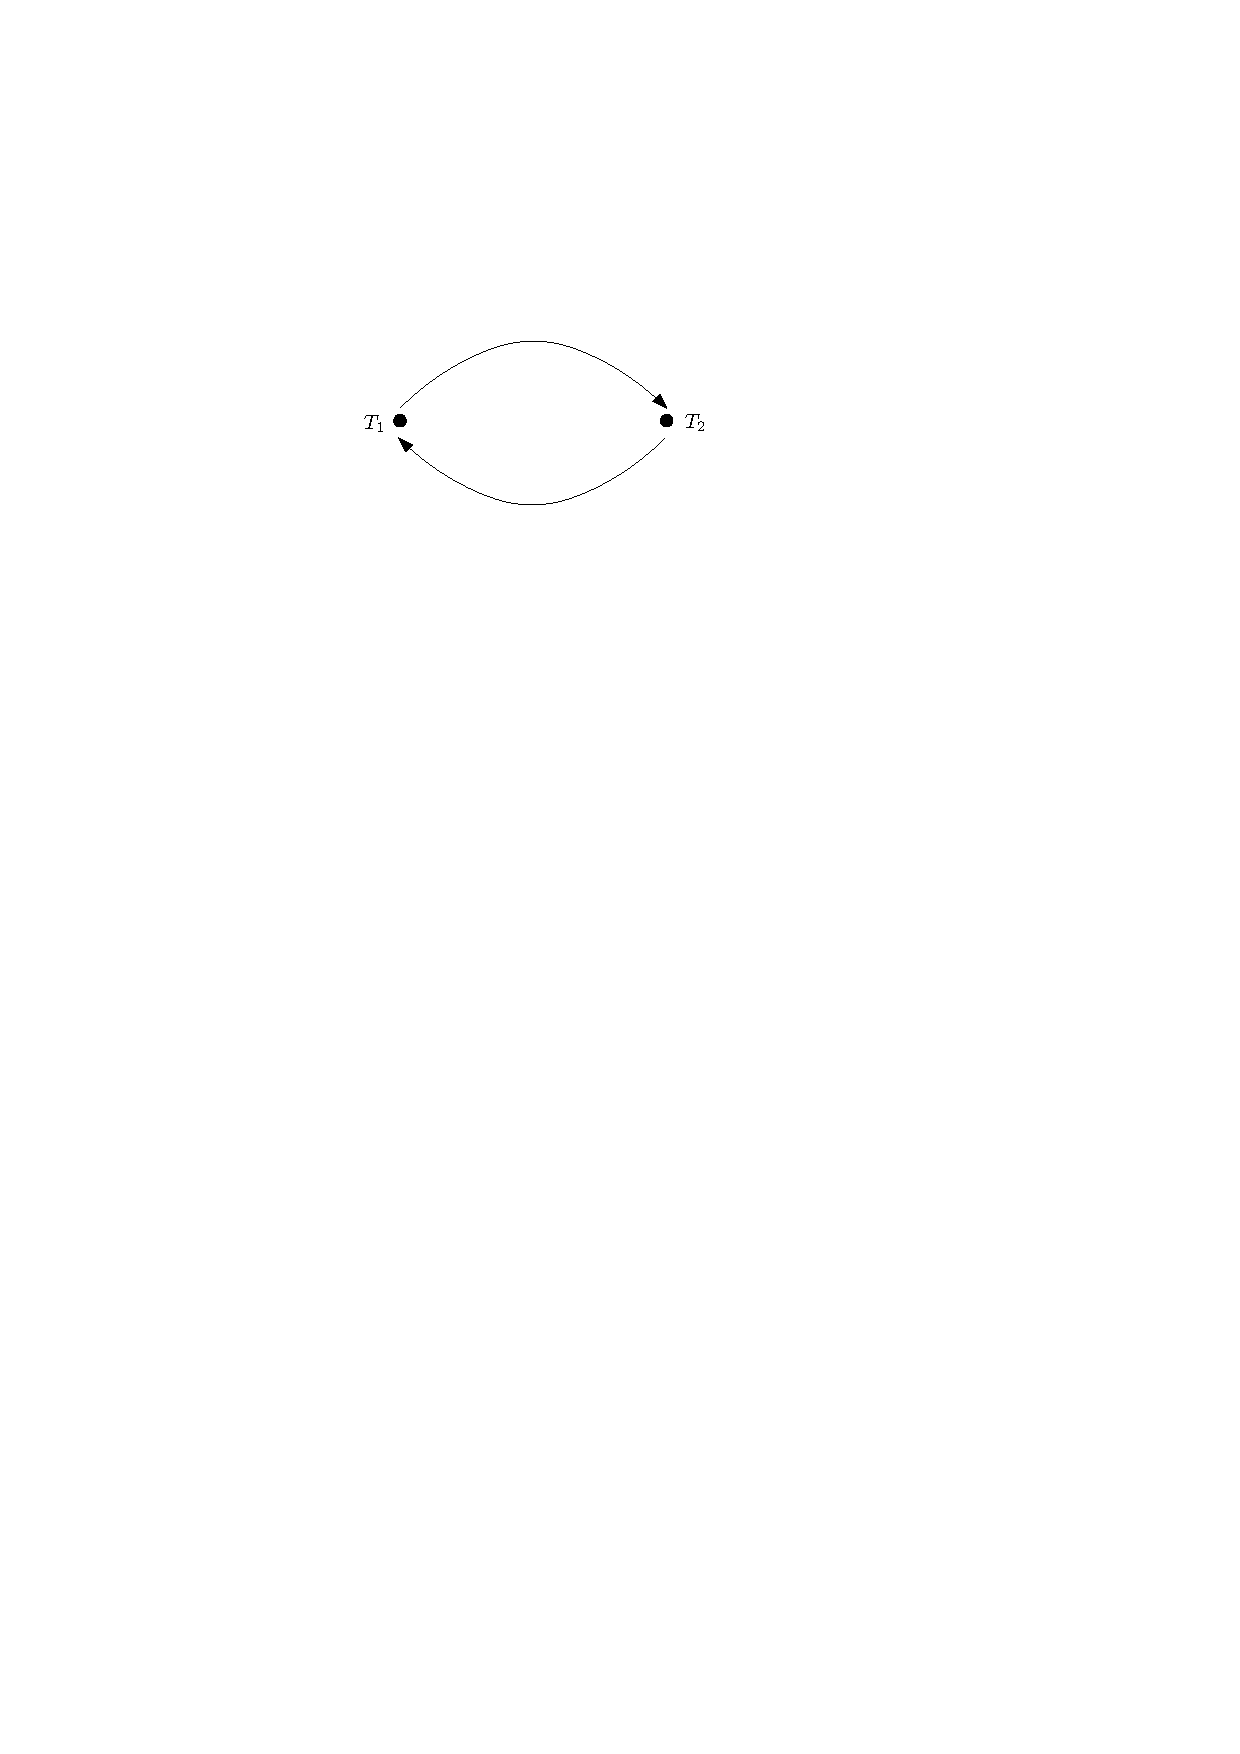
\includegraphics[height=15mm]{./artwork/pg1}
                \end{center}
            \end{minipage}
        \end{tabular}

        \vgap

        Instructions 1 and 6 are in conflict. \\
        Instructions 3 and 5 are in conflict. \\
        Instructions 5 and 6 are in conflict.
    }
}
%-------------------------------------------------------------
\myfrm{
    \cbox{green}{
        \blue{Example:}

        \vgap

        \begin{tabular}{cc}
            \hspace{-5mm}
            \begin{minipage}{0.57\linewidth}
                \begin{tabular}{c|c|c|c}
                    &$\red{T_1}$ & $\red{T_2}$ & $\red{T_3}$ \\
                    \hline
                    1&&\rd($A$) & \\
                    2&$\rd(B)$ &\\
                    3&&\wt($A$) & \\
                    4&&& $\rd(A)$ \\
                    5&\wt($B$) & & \\
                    6&&& \wt($A$) \\
                    7&&$\rd(B)$ & \\
                    8&&$\wt(B)$ & \\
                    9&\cmt&& \\
                    10&& \cmt & \\
                    11&&& \cmt
                \end{tabular}
            \end{minipage}
            &
            \hspace{5mm}
            \begin{minipage}{0.37\linewidth}
                \begin{center}
                    Precedence graph: \\[3mm]
                    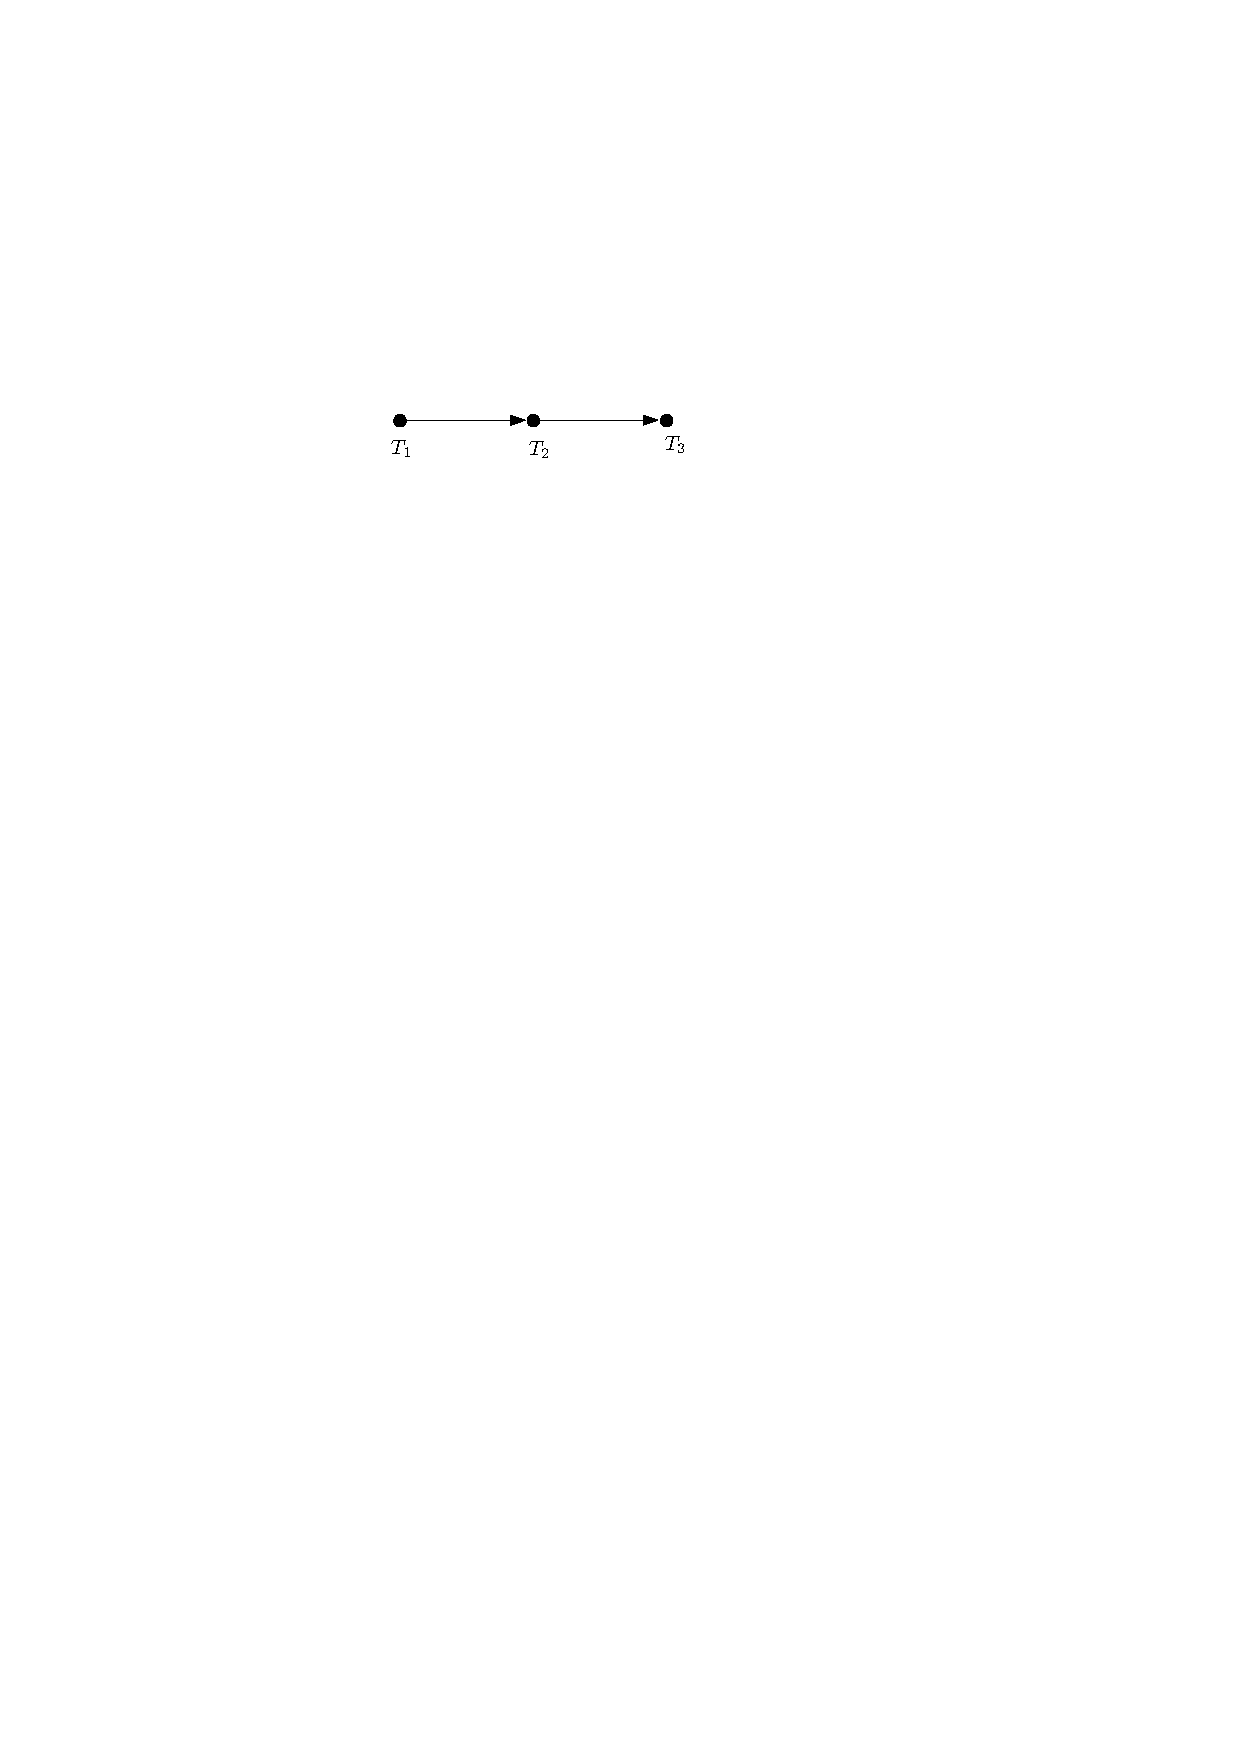
\includegraphics[height=5mm]{./artwork/pg2}
                \end{center}
            \end{minipage}
        \end{tabular}

    }
}
%-------------------------------------------------------------
\myfrm{
    \xmybox{Conflict Serializability}

    %\vgap

    \cbox{blue}{
        A schedule is \blue{conflict serializable}\\ if its precedence graph contains no cycles.
    }

    \cbox{green}{
        \blue{Example:}

        %\vspace{-1mm}

        \begin{tabular}{cc}
            \hspace{-5mm}
            \begin{minipage}{0.57\linewidth}
                \begin{tabular}{c|c|c|c}
                    &$\red{T_1}$ & $\red{T_2}$ & $\red{T_3}$ \\
                    \hline
                    1&&\rd($A$) & \\
                    2&$\rd(B)$ &\\
                    3&&\wt($A$) & \\
                    4&&& $\rd(A)$ \\
                    5&\wt($B$) & & \\
                    6&&& \wt($A$) \\
                    7&&$\rd(B)$ & \\
                    8&&$\wt(B)$ & \\
                    9&\cmt&& \\
                    10&& \cmt & \\
                    11&&& \cmt
                \end{tabular}
            \end{minipage}
            &
            \hspace{5mm}
            \begin{minipage}{0.37\linewidth}
                \begin{center}
                    Precedence graph: \\[3mm]
                    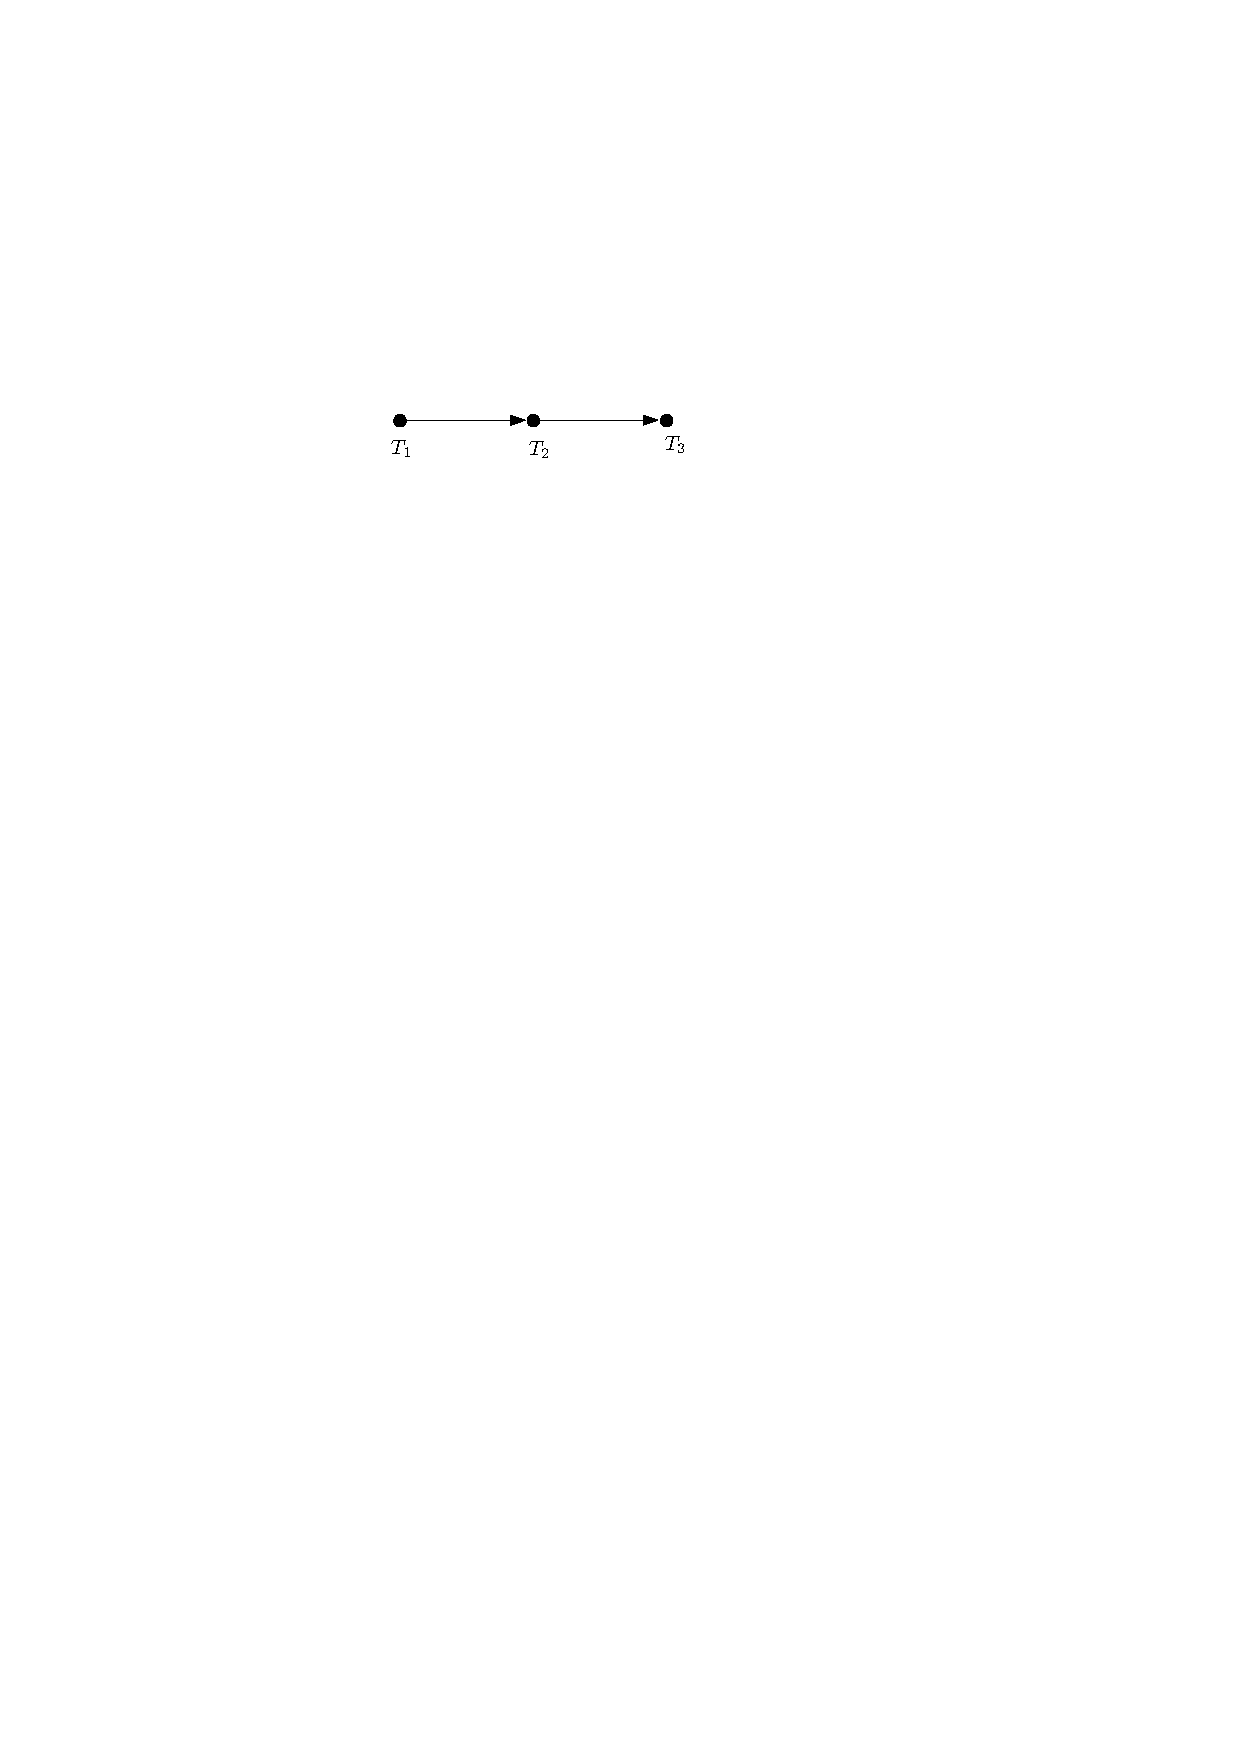
\includegraphics[height=5mm]{./artwork/pg2} \\
                    \bred{Conflict serializable}
                \end{center}
            \end{minipage}
        \end{tabular}

    }
}
%-------------------------------------------------------------
\myfrm{
    \cbox{green}{
        \blue{Example:}

        \vgap

        \begin{tabular}{cc}
            \begin{minipage}{0.47\linewidth}
                \begin{tabular}{c|c|c}
                    &$\red{T_1}$ & $\red{T_2}$\\
                    \hline
                    1&\rd($A$) & \\
                    2&$A = A + 1$ &\\
                    3&& \rd($A$) \\
                    4&& $A = A + 1$ \\
                    5&\wt($A$) & \\
                    6&& \wt($A$) \\
                    7&& \cmt \\
                    8&\cmt &
                \end{tabular}
            \end{minipage}
            &
            \begin{minipage}{0.47\linewidth}
                \begin{center}
                    Precedence graph: \\[1mm]
                    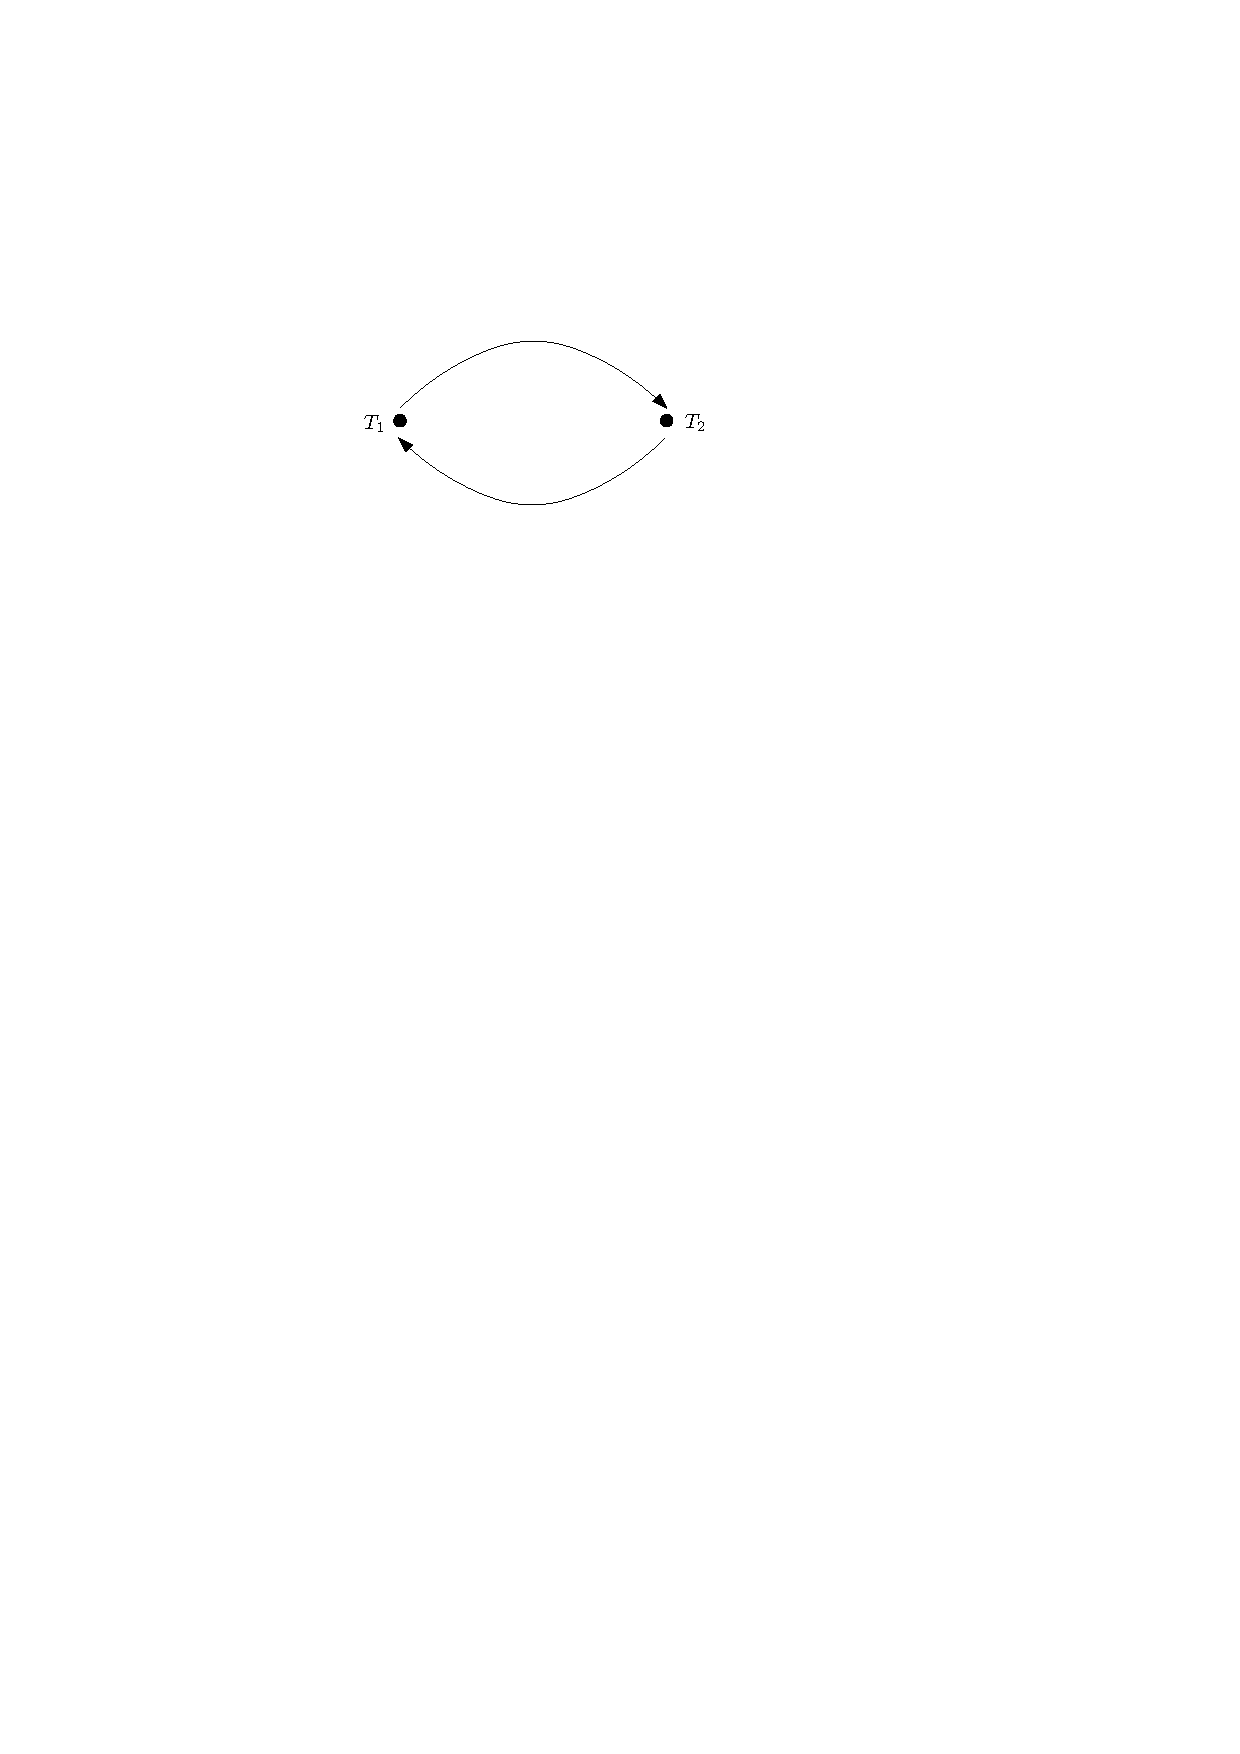
\includegraphics[height=15mm]{./artwork/pg1}\\
                    \bred{Not} conflict serializable
                \end{center}
            \end{minipage}
        \end{tabular}
    }
}
%-------------------------------------------------------------
\myfrm{
    \cbox{blue}{
        \blue{Theorem:} A conflict-serializable schedule must be serializable.
    }

    \vgap

    \cbox{green}{
        \blue{Fact:} It is always possible to convert a conflict-serializable schedule to a serializable one by swapping non-conflicting instructions.
    }
}
%-------------------------------------------------------------
\myfrm{
    \cbox{green}{
        \blue{Example:}

        \begin{center}
                \begin{tabular}{c|c|c|c}
                    &$\red{T_1}$ & $\red{T_2}$ & $\red{T_3}$ \\
                    \hline
                    1&&\rd($A$) & \\
                    2&$\rd(B)$ &\\
                    3&&\wt($A$) & \\
                    4&&& $\rd(A)$ \\
                    5&\wt($B$) & & \\
                    6&&& \wt($A$) \\
                    7&&$\rd(B)$ & \\
                    8&&$\wt(B)$ & \\
                    9&\cmt&& \\
                    10&& \cmt & \\
                    11&&& \cmt
                \end{tabular}
        \end{center}

        Try converting the above schedule to the serial schedule $(T_1,$ $T_2,$ $T_3)$ by swapping non-conflicting instructions.

        \cbox{red}{
            \blue{Think:} Is it possible to convert it to $(T_2, T_1, T_3)$?
        }
     }
}
%-------------------------------------------------------------
\myfrm{
    As mentioned, conflict-serializability implies serializability. \\
    Is the opposite also true? The answer is: \bred{no}.

    \vgap

    \cbox{green}{
        \blue{Example:}

        \begin{center}
        \begin{tabular}{c|c|c}
            & $\red{T_1}$ & $\red{T_2}$\\
            \hline
            1& $A = 0$ & \\
            2& \wt($A$) & \\
            3& & $A = 1$ \\
            4&& $\wt(A)$ \\
            5& $A = 2$ & \\
            6& $\wt(A)$ & \\
            7&& \cmt \\
            8&\cmt &
        \end{tabular}
        \end{center}

        The schedule is serializable because it is equivalent to the serial schedule $(T_2, T_1)$, but it is \bred{not} conflict-serializable.
    }
}
%-------------------------------------------------------------
\myfrm{
    \cbox{blue}{
        To enforce the serializable isolation level, the existing database systems achieve the purpose by ensuring conflict serializability instead. As we will see later in the course, there are effective protocols to general conflict serializable schedules.
    }
}
%-------------------------------------------------------------
\myfrm{
    \cbox{yellow}{
        \centering
        The content of the rest slides will not be tested.
    }
}
%-------------------------------------------------------------
\myfrm{
    Recall:
    \cbox{blue}{
        A \blue{phantom} refers to the situation where executing the same query twice returns different results even though the transaction performs no  modifications on the relevant data.
    }

    \cbox{green}{
        \blue{Example:} Relation $R(X, Y)$.

        \begin{center}
        \begin{tabular}{c|c}
            $\red{T_1}$ & $\red{T_2}$\\
            \hline
            find all $t \in R$ with $\red{t.X = 1}$ & \\
            & $\ins$ tuple $(1, y)$ in $R$ \\
            find all $t \in R$ with $\red{t.X = 1}$ & \\
            & \cmt \\
            \cmt &
        \end{tabular}
        \end{center}
    }

    \cbox{red}{
        Is the above schedule conflict-serializable?
    }
}
%-------------------------------------------------------------
\myfrm{
    \cbox{green}{
        \blue{Example:} Relation $R(X, Y)$.

        \begin{center}
        \begin{tabular}{c|c|c}
            &$\red{T_1}$ & $\red{T_2}$\\
            \hline
            1&find all $t \in R$ with $\red{t.X = 1}$ & \\
            2&& $\ins$ tuple $(1, y)$ in $R$ \\
            3&find all $t \in R$ with $\red{t.X = 1}$ & \\
            4&& \cmt \\
            5&\cmt &
        \end{tabular}
        \end{center}
    }

    \cbox{red}{
        Is the above schedule conflict-serializable? \bred{Answer:} No.

        \vgap

        Instructions 1 and 2 are in conflict (as explained in the next slide). \\
        Instructions 2 and 3 are in conflict.

        \vgap

        Hence, the precedence graph contains a cycle.
    }
}
%-------------------------------------------------------------
\myfrm{
    \cbox{green}{
        \blue{Example:} Relation $R(X, Y)$.

        \begin{center}
        \begin{tabular}{c|c|c}
            &$\red{T_1}$ & $\red{T_2}$\\
            \hline
            1&find all $t \in R$ with $\red{t.X = 1}$ & \\
            2&& $\ins$ tuple $(1, y)$ in $R$ \\
            3&find all $t \in R$ with $\red{t.X = 1}$ & \\
            4&& \cmt \\
            5&\cmt &
        \end{tabular}
        \end{center}
    }

    \cbox{blue}{
        Instructions 1 and 2 are in conflict. \blue{Why?}

        \vgap

        Instruction 1 reads every tuple $t \in R$ satisfying the condition $t.X = 1$. The tuple $(1, y)$ inserted by $T_2$ qualifies for the condition.
    }
}
%-------------------------------------------------------------
\end{document} 



